\subsection{Caso d'uso UC 1: Utilizzo di bolle predefinite disponibili nell'SDK}
\label{Caso d'uso UC 1: Utilizzo di bolle predefinite disponibili nell'SDK}
\begin{figure}[ht]
	\centering
	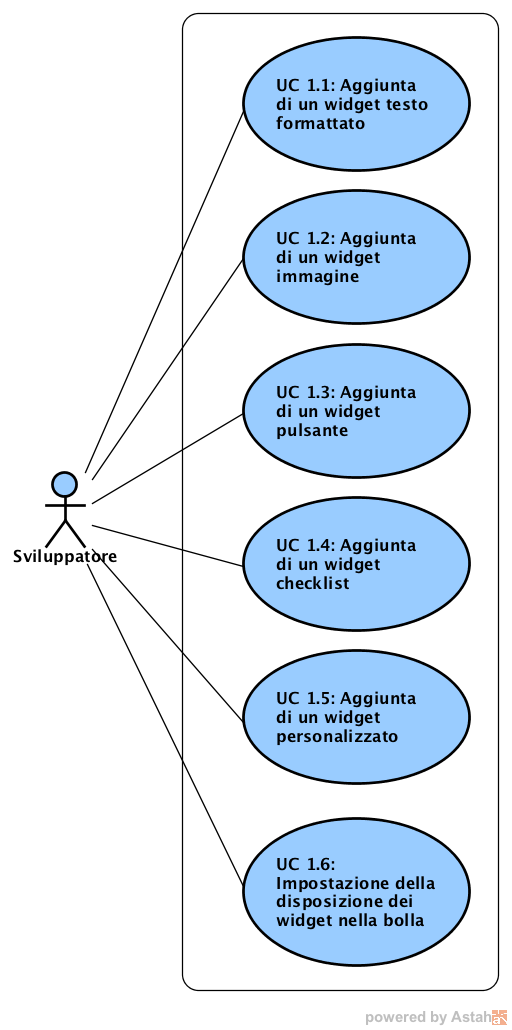
\includegraphics[scale=0.80]{Usecases/img/UC1.png}
	\caption{Caso d'uso UC 1: Utilizzo di bolle predefinite disponibili nell'SDK}
\end{figure}

\FloatBarrier
\begin{itemize}
\item \textbf{Attori:} Sviluppatore;
\item \textbf{Descrizione:} Tramite l'\termine{SDK} lo sviluppatore vuole:
	\begin{itemize}
	\item{Utilizzare una bolla di tipo testo formattato.} 
	\item{Utilizzare una bolla di tipo bottone.}
	\item{Utilizzare una bolla di tipo checklist.}
	\item{Utilizzare una bolla di tipo immagine.}
	\item{Modificare un istanza di una bolla concreta.}
	\item{Utilizzare una bolla vuota.}
	\end{itemize} 
\item \textbf{Precondizione:} Lo sviluppatore ha accesso all'\termine{SDK}.
\item \textbf{Postcondizione:} Lo sviluppatore ha creato del codice eseguibile. 
\item \textbf{Scenario principale:}
	\begin{itemize}
	\item{Lo sviluppatore vuole utilizzare una bolla di tipo testo formattato (UC 1.1).}
	\item{Lo sviluppatore vuole utilizzare una bolla di tipo bottone (UC 1.2).}
	\item{Lo sviluppatore vuole utilizzare una bolla di tipo checklist (UC 1.3).}
	\item{Lo sviluppatore vuole utilizzare una bolla di tipo immagine (UC 1.4).}
	\item{Lo sviluppatore vuole modificare un'istanza di una bolla concreta, modificandone gli attributi (UC 1.5).}
	\item {Lo sviluppatore vuole utilizzare una bolla vuota (UC 1.6).}
	\end{itemize}
\end{itemize}